\documentclass[no-math]{ctexbeamer}
\usepackage{Buct}

\author[蓝青]{蓝青 \and 李四~教授}
\title{一份很简短的 BUCT Beamer Theme 介绍}
\subtitle{申请北京化工大学工学硕士学位}
\institute[CMSE of BUCT]{北京化工大学\quad 材料科学与工程学院}
\date{\today}

\begin{document}

%\kaishu
\begin{frame}
	\titlepage
	\begin{figure}[htpb]
		\begin{center}
			
\includegraphics[width=0.15\linewidth]{pic/BUCT-badge.pdf}
		\end{center}
	\end{figure}
\end{frame}

\begin{frame}
	\tableofcontents[sectionstyle=show,subsectionstyle=show/shaded/hide,subsubsectionstyle=show/shaded/hide]
\end{frame}


\section{课题背景}

\begin{frame}{这份 Beamer 模板是什么?}
	\begin{itemize}[<+-| alert@+>] % 当然,除了alert,手动在里面插 \pause 也行,见后
		\item 这是北京化工大学的非官方 Beamer 模板,魔改自 \href{https://www.overleaf.com/latex/templates/thu-beamer-theme/vwnqmzndvwyb}{THU Beamer Theme}。
		\item 中文支持请选择 \XeLaTeX 编译选项,\emph{不支持 CTeX 套装}。
		\item 本文档即为示例文件,推荐结合源代码看一看。
		\item 项目地址位于 \href{https://github.com/Miracle0565/buct-Beamer-Theme}{GitHub},欢迎反馈。
	\end{itemize}
\end{frame}


\section{研究现状}

\subsection{Beamer主题分类}

\begin{frame}
	\begin{itemize}
		\item 有一些随 \TeX\ Live 发布,例如 Xiaoshan(萧山)。\pause
		\item 其他同学制作的北化 Beamer,适用于 $16:9$ 的比例,位于 \href{https://cn.overleaf.com/latex/templates/beamer-for-buct/rndypbwvfxrp}{Overleaf} 或 \href{https://github.com/Livioni/Beamer-Temlate-for-BUCT}{GitHub}。\pause
		\item Overleaf 和 GitHub 上也能找到许多其他风格的模板,可根据喜好自行选用。
	\end{itemize}
\end{frame}


\section{研究内容}

\subsection{字体}
\begin{frame}
	\begin{enumerate}
		\item 中文字体:优先使用思源黑体\footnote{下载:\href{https://mirrors.tuna.tsinghua.edu.cn/adobe-fonts/source-han-sans/OTF/SimplifiedChinese/}{清华大学镜像站} 或者 \href{https://mirror.nju.edu.cn/adobe-fonts/source-han-sans/OTF/SimplifiedChinese/}{南京大学镜像站}},如果不存在将使用默认设置。本模板使用 Regular 和 Bold 两种字重。
		\item 英文字体:使用 Fira 系列字体,其已集成于 TeX Live 中,故无需另行下载。
	\end{enumerate}
\end{frame}

\subsection{中文示例}

\begin{frame}{临江仙·滚滚长江东逝水}
	\begin{itemize}
		\item 滚滚长江东逝水,浪花淘尽英雄。是非成败转头空。\emph{青山依旧在,几度夕阳红。}
		\item 白发渔樵江渚上,惯看秋月春风。一壶浊酒喜相逢。古今多少事,都付笑谈中。
		\item 滾滾長江東逝水,浪花淘盡英雄。是非成敗轉頭空。\emph{青山依舊在,幾度夕陽紅。}
		\item 白髮漁樵江渚上,慣看秋月春風。一壺濁酒喜相逢。古今多少事,都付笑談中。
	\end{itemize}
\end{frame}

\subsection{Examples in English}

\begin{frame}{from The Book of Mozilla}
	\begin{itemize}
		\item And the beast shall come forth \emph{surrounded by a roiling cloud of vengeance.} The house of the unbelievers shall be razed and they shall be scorched to the earth. Their tags shall blink until the end of days.
		\item And the beast shall be made legion. Its numbers shall be increased a thousand thousand fold. The din of a million keyboards like unto a great storm shall cover the earth, \textit{and the followers of Mammon shall tremble.}
	\end{itemize}
\end{frame}

\subsection{其他例子}

\begin{frame}{表格}
	\begin{table}[h]
		\centering
		\begin{tabular}{ll}
			\toprule
			Microsoft\textsuperscript{\textregistered}  Word & \LaTeX \\
			\midrule
			文字处理工具 & 专业排版软件 \\
			容易上手,简单直观 & 容易上手 \\
			所见即所得 & 所见即所想,所想即所得 \\
			高级功能不易掌握 & 进阶难,但一般用不到 \\
			处理长文档需要丰富经验 & 和短文档处理基本无异 \\
			花费大量时间调格式 & 无需担心格式,专心作者内容 \\
			公式排版差强人意 & 尤其擅长公式排版 \\
			二进制格式,兼容性差 & 文本文件,易读、稳定 \\
			付费商业许可 & 自由免费使用 \\
			\bottomrule
		\end{tabular}
	\end{table}
\end{frame}

\begin{frame}{公式}
	\begin{exampleblock}{无编号公式} % 加 *
		\begin{equation*}
			J(\theta) = \mathbb{E}_{\pi_\theta}[G_t] = \sum_{s\in\mathcal{S}} d^\pi (s)V^\pi(s)=\sum_{s\in\mathcal{S}} d^\pi(s)\sum_{a\in\mathcal{A}}\pi_\theta(a|s)Q^\pi(s,a)
		\end{equation*}
	\end{exampleblock}
	
	\begin{exampleblock}{多行多列公式\footnote{如果公式中有文字出现,请用 \cmd{text\{\}} 包含}}
		% 使用 & 分隔
		\begin{align}
			Q_\text{target}&=r+\gamma Q^\pi(s^\prime, \pi_\theta(s^\prime)+\epsilon)\\
			\epsilon&\sim\text{clip}(\mathcal{N}(0, \sigma), -c, c)\nonumber
		\end{align}
	\end{exampleblock}
\end{frame}

\begin{frame}
	\begin{exampleblock}{编号多行公式}
		% Taken from Mathmode.tex
		\begin{multline}
			A=\lim_{n\rightarrow\infty}\Delta x\left(a^{2}+\left(a^{2}+2a\Delta x+\left(\Delta x\right)^{2}\right)\right.\label{eq:reset}\\
			+\left(a^{2}+2\cdot2a\Delta x+2^{2}\left(\Delta x\right)^{2}\right)\\
			+\left(a^{2}+2\cdot3a\Delta x+3^{2}\left(\Delta x\right)^{2}\right)\\
			+\ldots\\
			\left.+\left(a^{2}+2\cdot(n-1)a\Delta x+(n-1)^{2}\left(\Delta x\right)^{2}\right)\right)\\
			=\frac{1}{3}\left(b^{3}-a^{3}\right)
		\end{multline}
	\end{exampleblock}
\end{frame}

\begin{frame}{Equations}
	\begin{itemize}
		\item Covariant derivative:
		\[
		\nabla \symbf{X} = \tensor{X}{^\alpha_{;\beta}} \pdv{x^\alpha} \otimes \dd{x^\beta}
						= \qty(\tensor{X}{^\alpha_{,\beta}} + \Gamma^{\alpha}_{\beta\gamma} \, X^\gamma) \,
							\pdv{x^\alpha} \otimes \dd{x^\beta}
		\]
		\item Einstein's field equations:
		\[ G_{\mu\nu} \equiv R_{\mu\nu} - \frac{1}{2} R g_{\mu\nu} = \frac{8\pi G}{c^4} T_{\mu\nu} \]
		\item Schwarzschild metric:
		\[
		c^2 \dd{\tau}^2 = \qty(1-\frac{r_{\mathrm{s}}}{r}) \, c^2 \dd{t}^2
						- \qty(1-\frac{r_{\mathrm{s}}}{r})^{-1} \dd{r}^2
						- r^2 \underbrace{\qty(\dd{\theta}^2 + \sin^2 \theta \dd{\varphi}^2)}_{\dd{\Omega}^2}
		\]
		\item Einstein--Hilbert action:
		\[ S = \frac{1}{2\kappa} \int R \sqrt{-g} \dd[4]{x} \]
	\end{itemize}
\end{frame}

\begin{frame}{图形与分栏}
	% From thuthesis user guide.
	\begin{minipage}[c]{0.3\linewidth}
		\psset{unit=0.8cm}
		\begin{pspicture}(-1.75,-3)(3.25,4)
			\psline[linewidth=0.25pt](0,0)(0,4)
			\rput[tl]{0}(0.2,2){$\vec e_z$}
			\rput[tr]{0}(-0.9,1.4){$\vec e$}
			\rput[tl]{0}(2.8,-1.1){$\vec C_{ptm{ext}}$}
			\rput[br]{0}(-0.3,2.1){$\theta$}
			\rput{25}(0,0){%
			\psframe[fillstyle=solid,fillcolor=lightgray,linewidth=.8pt](-0.1,-3.2)(0.1,0)}
			\rput{25}(0,0){%
			\psellipse[fillstyle=solid,fillcolor=yellow,linewidth=3pt](0,0)(1.5,0.5)}
			\rput{25}(0,0){%
			\psframe[fillstyle=solid,fillcolor=lightgray,linewidth=.8pt](-0.1,0)(0.1,3.2)}
			\rput{25}(0,0){\psline[linecolor=red,linewidth=1.5pt]{->}(0,0)(0.,2)}
%           \psRotation{0}(0,3.5){$\dot\phi$}
%           \psRotation{25}(-1.2,2.6){$\dot\psi$}
			\psline[linecolor=red,linewidth=1.25pt]{->}(0,0)(0,2)
			\psline[linecolor=red,linewidth=1.25pt]{->}(0,0)(3,-1)
			\psline[linecolor=red,linewidth=1.25pt]{->}(0,0)(2.85,-0.95)
			\psarc{->}{2.1}{90}{112.5}
			\rput[bl](.1,.01){C}
		\end{pspicture}
	\end{minipage}\hspace{1cm}
	\begin{minipage}{0.5\linewidth}
		\medskip
		%\hspace{2cm}
		\begin{figure}[h]
			\centering
			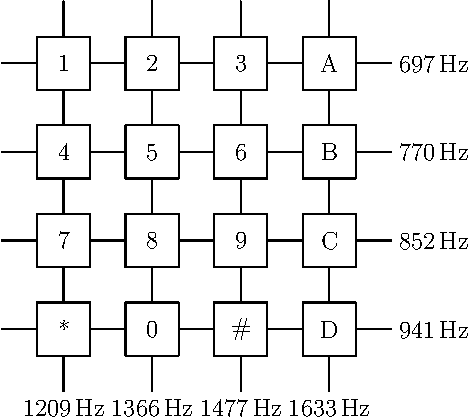
\includegraphics[height=.4\textheight]{pic/dtmf.pdf}
		\end{figure}
	\end{minipage}
\end{frame}

\begin{frame}[fragile]{\LaTeX{} 常用命令}
	\begin{exampleblock}{命令}
		\centering
		\footnotesize
		\begin{tabular}{llll}
			\cmd{chapter} & \cmd{section} & \cmd{subsection} & \cmd{paragraph} \\
			章 & 节 & 小节 & 带题头段落 \\\hline
			\cmd{centering} & \cmd{emph} & \cmd{verb} & \cmd{url} \\
			居中对齐 & 强调 & 原样输出 & 超链接 \\\hline
			\cmd{footnote} & \cmd{item} & \cmd{caption} & \cmd{includegraphics} \\
			脚注 & 列表条目 & 标题 & 插入图片 \\\hline
			\cmd{label} & \cmd{cite} & \cmd{ref} \\
			标号 & 引用参考文献 & 引用图表公式等\\\hline
		\end{tabular}
	\end{exampleblock}
	\begin{exampleblock}{环境}
		\centering
		\footnotesize
		\begin{tabular}{lll}
			\env{table} & \env{figure} & \env{equation}\\
			表格 & 图片 & 公式 \\\hline
			\env{itemize} & \env{enumerate} & \env{description}\\
			无编号列表 & 编号列表 & 描述 \\\hline
		\end{tabular}
	\end{exampleblock}
\end{frame}

\begin{frame}[fragile]{\LaTeX{} 环境命令举例}
	\begin{minipage}{0.5\linewidth}
\begin{lstlisting}[language=TeX]
\begin{itemize}
  \item A \item B
  \item C
  \begin{itemize}
    \item C-1
  \end{itemize}
\end{itemize}
\end{lstlisting}
	\end{minipage}\hspace{1cm}
	\begin{minipage}{0.3\linewidth}
		\begin{itemize}
			\item A
			\item B
			\item C
			\begin{itemize}
				\item C-1
			\end{itemize}
		\end{itemize}
	\end{minipage}
	\medskip
	\pause
	\begin{minipage}{0.5\linewidth}
\begin{lstlisting}[language=TeX]
\begin{enumerate}
  \item 巨佬 \item 大佬
  \item 萌新
  \begin{itemize}
    \item[n+e] 瑟瑟发抖
  \end{itemize}
\end{enumerate}
\end{lstlisting}
	\end{minipage}\hspace{1cm}
	\begin{minipage}{0.3\linewidth}
		\begin{enumerate}
			\item 巨佬
			\item 大佬
			\item 萌新
			\begin{itemize}
				\item[n+e] 瑟瑟发抖
			\end{itemize}
		\end{enumerate}
	\end{minipage}
\end{frame}

\begin{frame}[fragile]{\LaTeX{} 数学公式}
	\begin{columns}
		\begin{column}{.55\textwidth}
\begin{lstlisting}[language=TeX]
$V = \frac{4}{3}\pi r^3$

\[
  V = \frac{4}{3}\pi r^3
\]

\begin{equation}
  \label{eq:vsphere}
  V = \frac{4}{3}\pi r^3
\end{equation}
\end{lstlisting}
		\end{column}
		\begin{column}{.4\textwidth}
			$V = \frac{4}{3}\pi r^3$
			\[
				V = \frac{4}{3}\pi r^3
			\]
			\begin{equation}
				\label{eq:vsphere}
				V = \frac{4}{3}\pi r^3
			\end{equation}
		\end{column}
	\end{columns}
\end{frame}

\begin{frame}[fragile]
	\begin{columns}
		\column{.6\textwidth}
\begin{lstlisting}[language=TeX]
\begin{table}[htbp]
    \caption{编号与含义}
    \label{tab:number}
    \centering
    \begin{tabular}{cl}
    \toprule
    编号 & 含义 \\
    \midrule
    1 & 4.0 \\
    2 & 3.7 \\
    \bottomrule
    \end{tabular}
\end{table}
公式~(\ref{eq:vsphere}) 的
编号与含义请参见
表~\ref{tab:number}。
\end{lstlisting}
		\column{.4\textwidth}
		\begin{table}[htpb]
			\centering
			\caption{编号与含义}
			\label{tab:number}
			\begin{tabular}{cl}\toprule
				编号 & 含义 \\\midrule
				1 & 4.0\\
				2 & 3.7\\\bottomrule
			\end{tabular}
		\end{table}
		\normalsize 公式~(\ref{eq:vsphere})的编号与含义请参见表~\ref{tab:number}。
	\end{columns}
\end{frame}

\begin{frame}{作图}
	\begin{itemize}
		\item 矢量图 eps, ps, pdf
		\begin{itemize}
			\item METAPOST, pstricks, pgf $\ldots$
			\item Xfig, Dia, Visio, Inkscape $\ldots$
			\item Matlab / Excel 等保存为 pdf
		\end{itemize}
		\item 标量图 png, jpg, tiff $\ldots$
		\begin{itemize}
			\item 提高清晰度,避免发虚
			\item 应尽量避免使用
		\end{itemize}
	\end{itemize}
	\begin{figure}[htpb]
		\centering
		
\includegraphics[width=0.2\linewidth]{pic/BUCT-badge.pdf}
		\caption{这个校徽就是矢量图}
	\end{figure}
\end{frame}

\section{计划进度}
\begin{frame}
	\begin{itemize}
		\item 一月:完成文献调研
		\item 二月:复现并评测各种Beamer主题美观程度
		\item 三、四月:美化BUCT Beamer主题
		\item 五月:论文撰写
	\end{itemize}
\end{frame}

\section{参考文献}

% 指明需罗列但正文中不引用的文献
\nocite{*}

\begin{frame}[allowframebreaks]
	% \tiny 用于调整字号,建议参考文献比较多的时候使用
	\tiny
	% 罗列参考文献列表使用 plain 格式,也可以用 GB/T 7714 的
	\bibliographystyle{plain}
	% 参考文献数据库,可以与 buctthesis 中的共用
	% 建议只罗列主要参考文献
	\bibliography{thesisbib}
\end{frame}

\begin{frame}
	\begin{center}
		{\huge
			Thank you for your attention!\\
			Questions?
		}
	\end{center}
\end{frame}

\end{document}